\documentclass{ccn}

\addbibresource{ccn_extended_abstract_refs.bib}

\title{Triangle Inequality Violations Reveal Context-Dependent Relational Re-Representation in a Large Language Model}

\author{Anonymous Authors}

\begin{document}

\maketitle

\begin{abstract}
Analogical reasoning depends on recognizing when different pairs instantiate
the same relation. Vector-space accounts explain this ability by representing
relations as difference vectors in a fixed metric space. On this view,
relational similarity judgments should satisfy triangle inequality. Behavioral
work, however, has shown selective violations of triangle inequality when an
ambiguous pair is compared across different relational contexts. These findings
suggest context dependence, but they do not reveal whether the effect arises
from response bias or from a genuine change in representation. We test this
question in Llama-3.1-70B, a vector-based system whose internal states can be
examined directly. We compare consistent cases, in which all comparisons
instantiate the same relation, with mixed cases, in which an ambiguous pair
participates in different relations across comparisons. The model reproduces
the human asymmetry: triangle inequality is largely preserved in consistent
cases but systematically violated in mixed cases. To probe the source of this
effect, we analyze condition-specific function vectors during in-context
learning and project them into a shared PCA space. In mixed contexts, the
representation associated with the ambiguous pair does not remain fixed, but
shifts toward different relational directions as sequential context changes.
These results suggest that the violation reflects context-sensitive
re-representation rather than a stable relational geometry with a biased
readout.
\end{abstract}

\section{Introduction}

Analogical reasoning depends on mapping common relations across superficially
different pairs. Whether those mappings reflect stable relational
representations or context-sensitive reconstruction is especially important for
vector-space accounts of analogy. These accounts explain analogy by
representing relations geometrically, often as difference vectors
\citep{Shepard1987}, and typically assume that each pair has a single
context-invariant representation. On that view, triangle inequality provides a
useful constraint: if relational similarity is derived from fixed positions in
a metric space, the constraint should hold. However, human judgments can
violate triangle inequality \citep{Tversky1977}, and analogous violations in
relational similarity arise especially in mixed-relation triangles, where one
pair can participate in different relations across comparison contexts
\citep{PetersonEtAl2020}. Behavioral data alone cannot determine whether this
pattern reflects response-level bias or a genuine change in the underlying
representation. Large language models provide a useful testbed because they
allow behavior and internal states to be examined within the same vector-based
system \citep{ToddEtAl2024}. We therefore ask whether Llama-3.1-70B shows the
same context-dependent pattern, and whether any such violation is accompanied
by systematic shifts in the model's internal representation of the same pair
across contexts.

\begin{figure}[ht]
  \begin{center}
    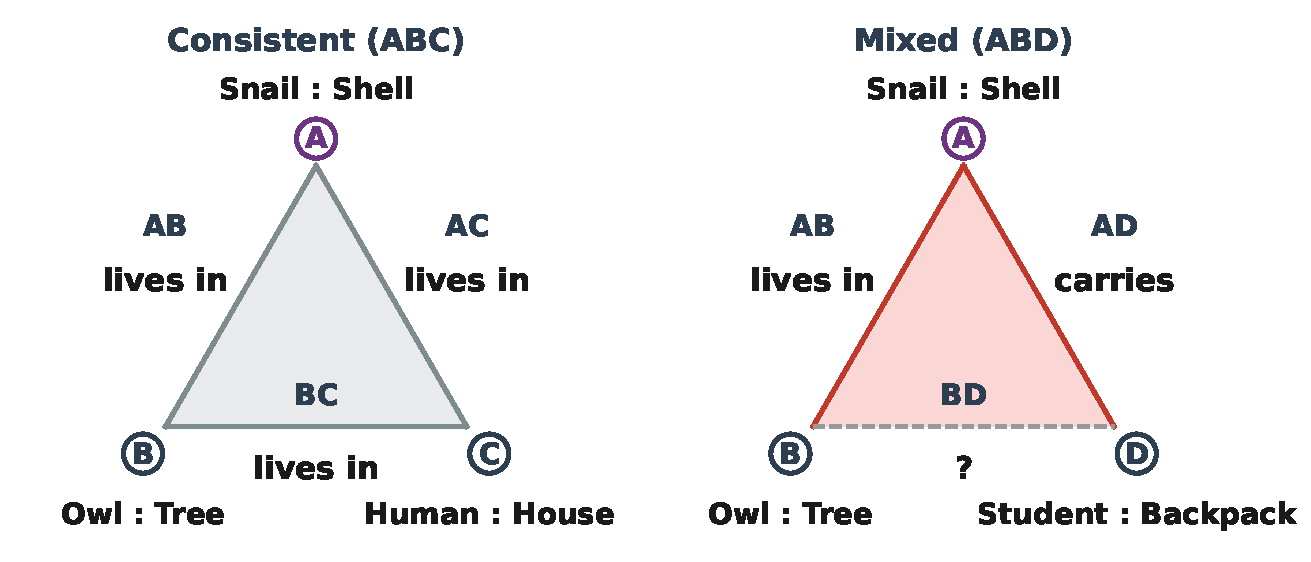
\includegraphics[width=\columnwidth]{figures/ccn_panel_a_triangle.pdf}
  \end{center}
  \caption{Stimulus design. Each item contains four pairs (A, B, C, D). Pair~A
  is ambiguous and defines a consistent triangle (ABC, left) where all edges
  share the same relation, and a mixed triangle (ABD, right) where A
  participates in different relations across comparisons.}
  \label{fig:design}
\end{figure}

\begin{figure*}[t]
  \centering
  \vspace*{-18pt}
  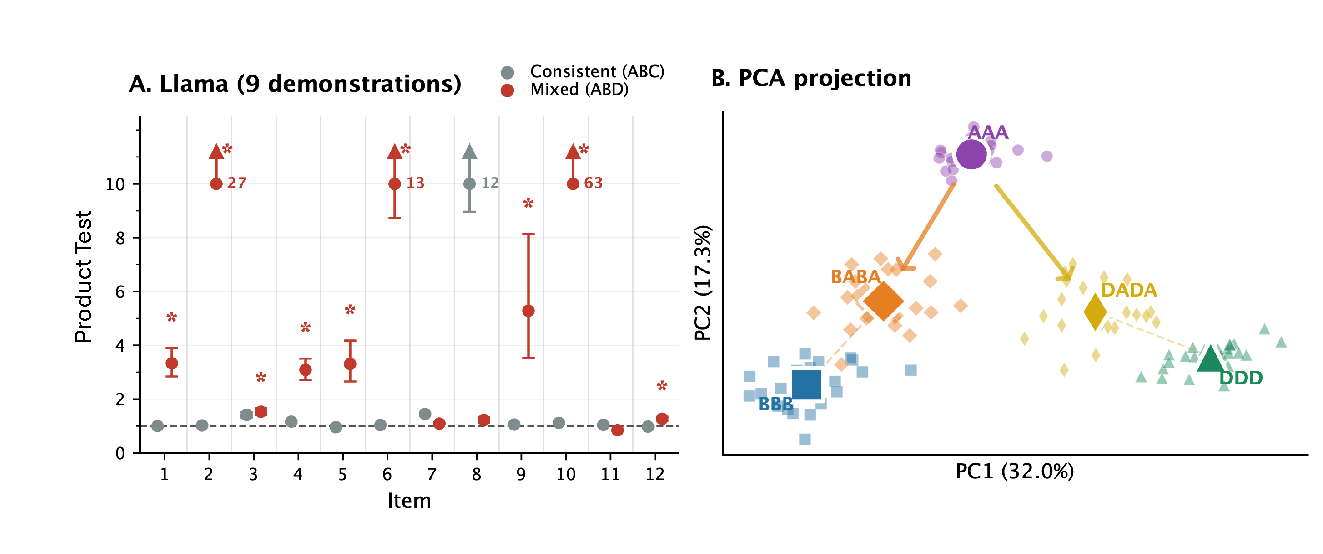
\includegraphics[width=\textwidth,trim=0 22 0 20,clip]{figures/figure3.pdf}
  \caption{LLM behavioral and representational results.
  \textbf{A}~Llama-3.1-70B with 9 in-context demonstrations shows higher
  mixed-triangle than consistent-triangle PT values across multiple items.
  \textbf{B}~In a shared PCA space (Q8), interleaved conditions shift toward
  different relational directions.}
  \label{fig:results}
\end{figure*}

\section{Methods}

The human experiment included 30 participants and 12 analogy items, each
containing four pairs labeled A, B, C, and D. Pair A was ambiguous, pair B
shared one relation with A, pair D shared the other, and pair C served as a
consistent control, yielding a consistent triangle (AB, AC, BC) and a mixed
triangle (AB, AD, BD). Human participants judged the relational similarity of
simple black clipart pairs on a 7-point Likert scale, with mirrored comparison
orders included to reduce order effects. Triangle inequality was assessed with a
symmetric product test \citep{PetersonEtAl2020}, with values above 1 indicating
violation. We rendered the same item structure as text word pairs and evaluated
it in Llama-3.1-70B using in-context Q/A prompts. In a pure/base five-edge
design, AB, AC, and AD were scored after A-family demonstrations, whereas BC
and BD were scored after B-family demonstrations, directly mirroring the two
human triangles. Each edge was evaluated across multiple shot conditions (1, 3,
5, 7, and 9 demonstrations), with the queried pair excluded from the
demonstrations so that scores reflected in-context generalization rather than
copying. The first-token log-probability of the correct target completion was
normalized within each question using a robust min-max transform (5th--95th
percentile, pooled across edges and shot conditions) before computing
product-test values for the consistent and mixed triangles.

To test whether this asymmetry was accompanied by a change in internal
representation rather than response bias alone, we conducted a separate
internal-state analysis across pure and interleaved in-context conditions (AAA,
BBB, BABA, DDD, and DADA). Using a fixed head set derived from prior
activation-patching analyses, we extracted for each trial a summed residual
contribution vector at the model state used to predict the first answer token.
Following the function-vector framework \citep{ToddEtAl2024}, we pooled these
trial-level vectors across conditions, fit a common PCA space, and summarized
each condition by its centroid in that shared space.

\section{Results}

Across the same 12 items, human judgments reproduced the established
asymmetry: the consistent triangle showed no reliable violations, whereas the
mixed triangle showed reliable violations in 6/12 items under a bootstrap
criterion ($P(\mathrm{PT}_{ABD} > 1) \ge .95$). In the 9-demonstration
analysis shown in Figure~\ref{fig:results}, Panel A, Llama-3.1-70B exhibited
the same directional asymmetry at the within-item comparison level:
$\mathrm{PT}_{ABD}$ significantly exceeded $\mathrm{PT}_{ABC}$ in 9/12 items
($\Delta \mathrm{PT} > 0,\, P \ge .95$). The remaining three items showed the
opposite pattern, and no item showed no reliable difference between the two
triangles. Thus, the model reproduced the human tendency for mixed-triangle
structure to yield larger product-test values than the consistent control.

The representational analysis showed a corresponding context-dependent
pattern. Figure~\ref{fig:results}, Panel B, shows Q8 as an illustrative
example (PC1 = 32.0\%, PC2 = 17.3\%). In the shared PCA space, pure
conditions formed separated centroids, whereas interleaved conditions shifted
the ambiguous pair toward different relation-specific endpoints: BABA lay
between AAA and BBB but closer to BBB, whereas DADA shifted from AAA toward
DDD. Qualitatively similar endpoint-directed reconfigurations were observed
across items. The ambiguous pair therefore did not remain at a fixed
representational location, but moved with sequential context.

\section{Discussion}

These findings argue against assuming a fixed representation for each pair in
standard vector-space accounts. The critical issue is not that vector geometry
cannot support relational similarity, but that context can dynamically
reconfigure the relevant representation before similarity is read out. This does
not treat LLMs as direct models of human cognition; rather, it tests a core
assumption of vector-space accounts in an explicit vector-space implementation.
For cognitive modeling, the implication is that relational similarity may
require context-dependent representational updating, not only static geometric
readout.

\clearpage
\printbibliography

\end{document}
